\documentclass[conference]{csce}

\usepackage[hmargin=.75in,vmargin=1in]{geometry}
\usepackage[american]{babel}
\usepackage[T1]{fontenc}
\usepackage{times}
\usepackage{caption}
\usepackage{url}

%%% Class name, option, and packages above are mandatory for generating an appropriate format 
%%% suitable for the CSCE style. Therefore, do not make any changes unless you know 
%%% what you are doing.
%%% However, if you need to use the subfig package, you must call it BEFORE the caption package.
%%% (NOTE: the subfig package probably will work but has not been tested.)

%%% The csce.cls is derived (in a quite dirty and quick manner) from the IEEEtrans.cls.
%%% At least the following packages are incompatible with the csce.cls:
%%% <DO NOT USE THEM> setspace, titlesec, amsthm
%%% There may be more, so if you use a package that produces a lot of errors or weird results, 
%%% be advised to avoid that package.

%%% Below packages are recommended to use for better results and compatible with the csce.cls
\usepackage{textcomp}
\usepackage{epsfig,graphicx}
\usepackage{xcolor}
\usepackage{amsfonts,amsmath,amssymb}
\usepackage{fixltx2e} % Fixing numbering problem when using figure/table* 
\usepackage{booktabs}

%%% Below packages are probably useful for some table-formatting purposes. Compatibility is not yet
%%% tested but probably fine.
%\usepackage{tabularx}
%\usepackage{tabulary}

%%% Using the hyperref package is not really necessary for conference papers, but if your paper includes
%%% a lot of URLs, and you wish them to be line-breakable, it might be useful.  When you need to use the
%%% hyperref package, make sure you set <colorlinks option> = true and all link colors black as shown in
%%% the sample below (the sample calls the ifpdf package, too).
%\usepackage{ifpdf} 
%\ifpdf
%\usepackage[pdftex,naturalnames,breaklinks=true,colorlinks=true,linkcolor=black,citecolor=black,filecolor=black,menucolor=black,urlcolor=black]{hyperref}
%\else
%\usepackage[dvips,naturalnames,breaklinks=true]{hyperref}
%\fi

\columnsep 6mm  %%% DO NOT CHANGE THIS


\title{\bf Pass a Note, Peek a Note - An AES Encrypted Messaging and Hacking Simulation System}          

%%%% Replace the author and institution/affiliation names. 
%%%% Make sure the author names are boldface.
\author{
{\bfseries Brandon Litwin}\\
Department of Computer Science, School of Computer Science and Mathematics\\
Marist College, 3399 North Road, Poughkeepsie, New York 12601\\
}

\begin{document}


\maketitle                        %%%% To set Title and Author names.


\begin{abstract}
AES is one of the best and most popular symmetric encryption algorithms designed to protect data. In this paper, I discuss the design of my Flask web page that implements AES in order to allow users to send encrypted messages to each other. In addition, encrypted messages will be sent to a third-party who selects the recipient to hack. It is the hacker's job to read the user's profile and extract their password from their personal information, which acts as an example of why users should complicate their passwords.
\end{abstract}


\vspace{1em}
\noindent\textbf{Keywords:}
 {\small  AES, symmetric encryption, cybersecurity, password cracking} 

%%%%%%%%%%%%%%%%%%%%%%%%%%%%%%%%%%%%%%%%%%%%%%%%%%%%%%%%%%%%


\section{Introduction}
Advanced Encryption Standard (AES) is a symmetric encryption algorithm that became a U.S. federal government standard in 2002. It has been praised for its efficiency and ease of implementation. Of course, a chain is only as strong as its weakest link. It does not matter how many bits an encryption key is or how many rounds an algorithm uses to generate its keys if a system has another vulnerability that is easily exploitable. \\
\indent My motivation comes from the simple idea of Alice and Bob, the cryptography couple, and Eve, their nosy neighbor. An example of this is depicted in Fig. \ref{fig:abe}. The idea of two people wanting to pass a message to each other and an unwanted third-party secretly trying to take a peek is the basis of all encryption algorithms, and is why my project is simply called Pass a Note, Peek a Note, or PaNPaN. \\
\begin{figure}
    \centering
    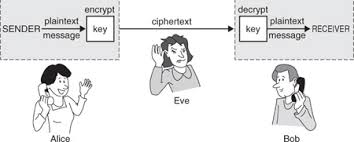
\includegraphics[width=\columnwidth]{AliceBobEve.jpeg}
    \caption{Alice wants to pass a note to Bob, but Eve is trying to peek!}
    \label{fig:abe}
\end{figure}
\indent In this paper, I will discuss my idea of an AES encrypted messaging system that is vulnerable to hacking. By demonstrating this system, I believe it will be clear how important defense-in-depth is and why we should use passwords that are not easy to crack from publicly available information. 

\section{Background and Other Work}
People have a history of using incredibly simple passwords. Passwords created by people are typically components of dictionary words and numbers that have a certain personal connection to them \cite{understanding passwords}. Most account creation systems encourage password complication by requiring a minimum length as well as a special character and number. People also follow simple rules to try and complicate them including, in order of frequency, concatenation, replacement, spelling mistake, and insertion \cite{understanding passwords}. If we can understand the process by which people create passwords, we can more easily determine how to crack them. 

\section{Methodology}
My system does not have people create passwords to protect their messages. Instead, it generates a password based on words found in the user's profile page. A sample user profile is shown in Fig \ref{fig:profile}. The user is told that their profile must contain at least three words that are at least four characters long. This is to ensure that the password is at least twelve characters long so it is not incredibly trivial to guess. The generated password is a simple lowercase concatenation of a random selection of these words. This is done to simulate an incredibly simple password that someone may create based on their personal information. \\
\begin{figure}
    \centering
    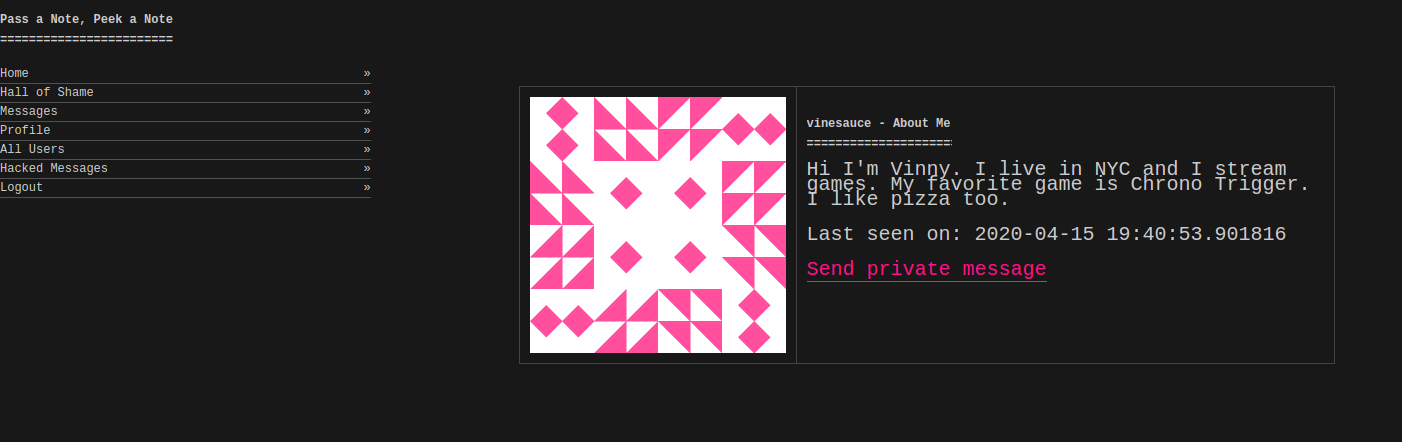
\includegraphics[width=\columnwidth]{profile.png}
    \caption{A sample user profile.}
    \label{fig:profile}
\end{figure}
\begin{figure}
    \centering
    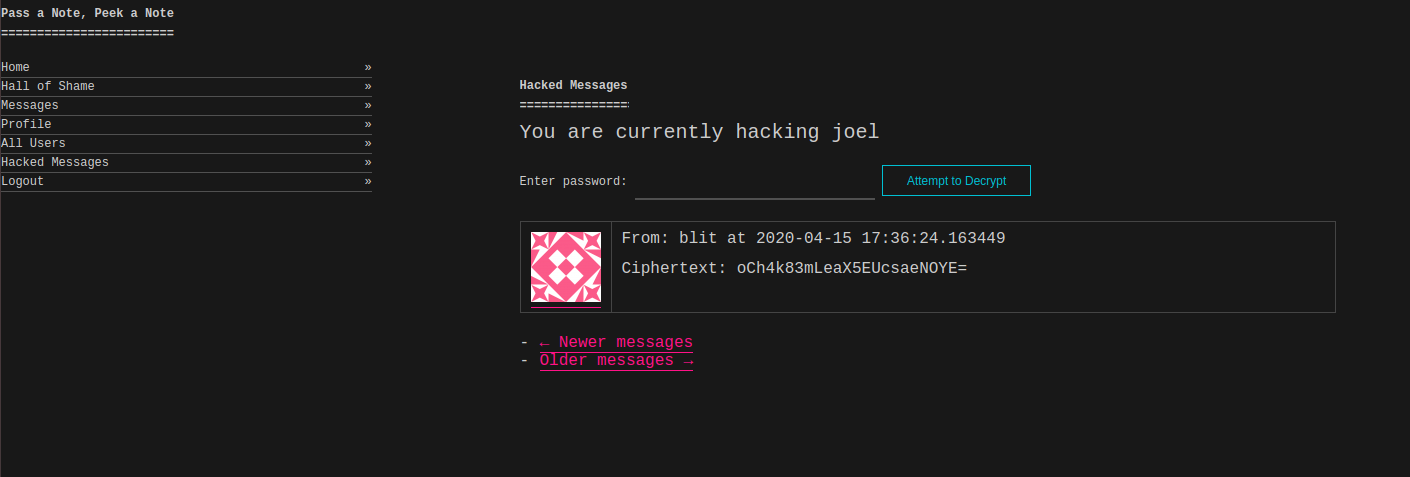
\includegraphics[width=\columnwidth]{before_hack.png}
    \caption{Hacker's view before the hack.}
    \label{fig:before}
\end{figure}
\begin{figure}
    \centering
    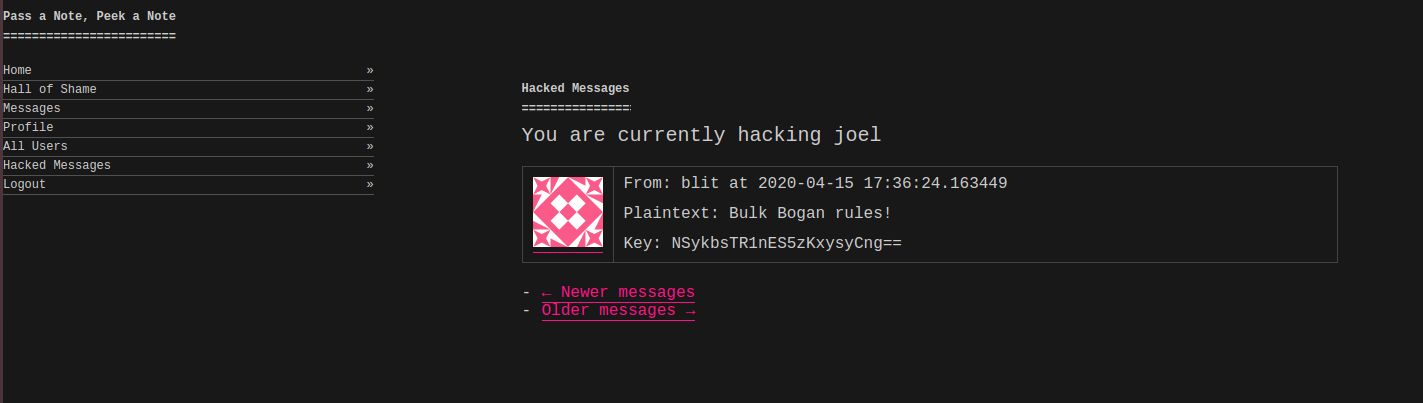
\includegraphics[width=\columnwidth]{after_hack.png}
    \caption{Hacker's view after the hack.}
    \label{fig:after}
\end{figure}
\indent During a hack, a hacker user will read through their chosen victim's profile. Since the rules of password generation are made public, the hacker understands that the password will be a combination of three words in that profile that are at least four characters long. When the hacker inputs the correct password, the user's message is displayed in plaintext, as well as the key that was used to decrypt the message. The hacker's view of the messages before a successful hack is shown in Fig. \ref{fig:before} and the view after a successful hack is shown in Fig. \ref{fig:after}.
\\ \indent The general use case of PaNPaN is as follows: 
\begin{enumerate}
    \item User creates an account.
    \item User writes some personal information in the "About Me" section of their profile.
    \item User clicks the password generation button to create a password to protect their messages.
    \item User sends a message to another user, which is AES encrypted.
    \item User chooses another user to hack and becomes a Hacker.
    \item Hacker receives all the messages from the user they chose to hack.
    \item Hacker attempts to brute-force the decryption password by using that user's public profile information.
    \item Upon successful hack, the victim is notified and their name is displayed on the Hall of Shame.
    \item The victim must edit their profile and generate a new password.\\
\end{enumerate}
\indent By gamifying the hacking process, hackers are encouraged to get creative in their password cracking. The system is built in such a way that it is very difficult for a user to not get hacked because they have very little influence in the way their passwords are generated. The point is to demonstrate that no matter how great an encryption algorithm like AES is, it means very little if there is another weak point in the system.
\section{AES Implementation}
The actual AES encryption is handled by the Python library Pycryptodome. When a user's message is sent, the message text is passed into an instance of an AES cipher from Pycryptodome's library. The AES class is able to take in a parameter to determine the mode of cipher to use. For this project, I chose to use CFB (Cipher FeedBack). As described in Pycryptodome's documentation, CFB mode performs an XOR operation from each byte of plaintext to a byte of the keystream. This mode was chosen because it makes it easy to pass in a message of any length without having to manually pad it to become a modulo of 16 bytes as a block cipher would require. The key for encryption is a randomly generated string of 16 bytes. An IV is generated through the Pycryptodome AES class's default iv method, which is later used for decryption. Next, a decryption cipher is created using the default decrypt method with the same key that was used for encryption and the IV from the previous step. The ciphertext is then passed into the decryption cipher to revert it back to plaintext. Both the ciphertext and plaintext of the message are stored into the database. This is done to save loading time of the web page during the actual hacking process. When a user's hack is successful, the page simply loads the plaintext message from the database and overwrites the encrypted text on the page.
\section{Results}
I was able to achieve all of the goals I set for this project. I have created a system that allows users to send AES encrypted messages to each other. The system allows each user to select another user that they wish to hack. The hacking works as described in the previous section, and the victim of the hack is notified to update their profile and generate a new password. Finally, I implemented the Hall of Shame page which displays the most successful hackers and the most attacked victims. The Hall of Shame is shown in Fig. \ref{fig:hos}. \\
\begin{figure}
    \centering
    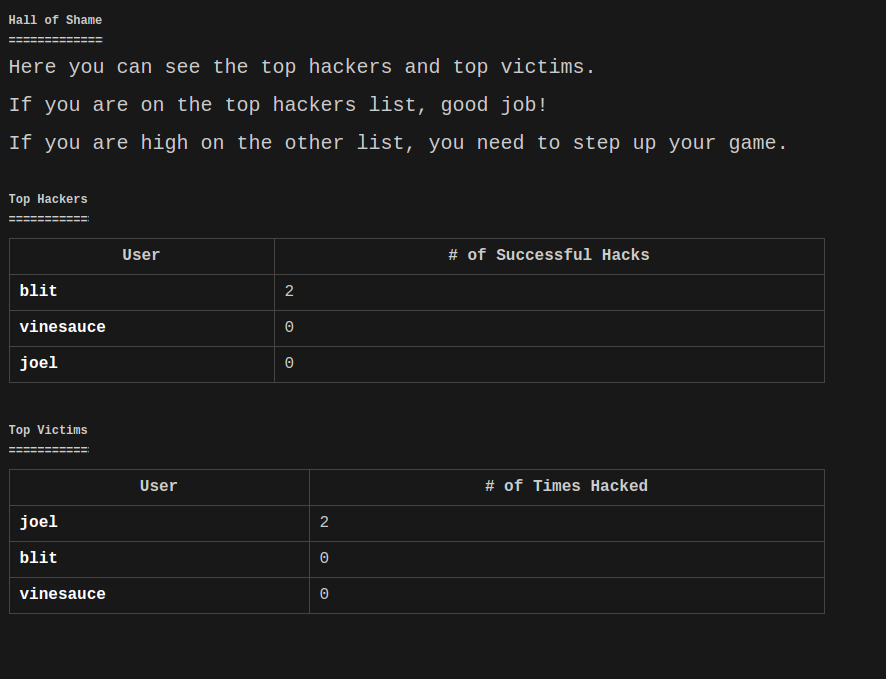
\includegraphics[width=\columnwidth]{hall_of_shame.png}
    \caption{You want to be among the top hackers, not the top victims.}
    \label{fig:hos}
\end{figure}

\section{Conclusion}
In this paper I discussed my motivation for Pass a Note, Peek a Note, the methodology by which I would create the system, and the results of the final implementation. I believe my system can be a fun and engaging way for those who are unfamiliar with hacking methods to get an introductory experience to basic password cracking. It also serves as a lesson in defense-in-depth. The well known cybersecurity principle, that a system is only as strong as its weakest length, is demonstrated here.\\

The Python code for this project has been made available at:
\begin{center}
    {\small \url{github.com/brandonlitwin/mscs630litwin.git}}
\end{center} 




%%%%%%%%%%%%%%%%%%%%%%%%%%%%%%%%%%%%%%%%%%%%%%%%%%%%%%%%%%%%
%%
%% Reference
%% Below is an example of bibliography that contains all entries within this document.
%% You can also let BibTeX generate your bibliography by inserting the following two commands:
%%
%% \bibliographystyle{IEEEtran}
%% \bibliography{<your_bibliography_file_1>,<your_bibliography_file_2>,...}
%%
%% Note that you need to make sure that LaTeX (BibTeX) can find IEEEtrans.bst in your system.
%% If you are unsure about that, just place IEEEtrans.bst in the same directory where your LaTeX source files reside.
%%
%%%%%%%%%%%%%%%%%%%%%%%%%%%%%%%%%%%%%%%%%%%%%%%%%%%%%%%%%%%%%
%%% Below thebibliography environment will be automatically created in a different file (your_file_name.bbl) 
%%% if you use BibTeX and specify IEEEtrans.bst.


\begin{thebibliography}{}
\providecommand{\newblock}{\relax}
%
% and use \bibitem to create references. Consult the Instructions
% for authors for reference list style.
%
\bibitem{understanding passwords}
Jakobsson, Markus, and Mayank Dhiman. \newblock {\em ``The benefits of understanding passwords.``} Mobile Authentication. Springer, New York, NY, 2013. 5-24.

\end{thebibliography}



\end{document}

